%! Author = itgramic
%! Date = 11.10.23

% Preamble
%\printglossary
{
    \hypersetup{hidelinks}
    \listoffigures
}
\pagestyle{headings}
\thispagestyle{fancy}
{
    \hypersetup{hidelinks}
%\thispagestyle{fancy}
    \listoftables
    \thispagestyle{fancy}
}
{
    \hypersetup{hidelinks}
    \lstlistoflistings
    \thispagestyle{fancy}
}
\pagestyle{headings}
\thispagestyle{fancy}
%\begin{thebibliography}{XX}
%    \bibitem[XY]{XY} blah
%\clearpage
%\thispagestyle{fancy}
{
%    \renewcommand*\printbibliography{\thispagestyle{fancy}}
    \cleardoublepage
%    \pagestyle{headings}
%    \thispagestyle{fancy}
%    \renewcommand{\bibname}{\thispagestyle{fancy}}
%    \renewcommand{\biblatex}{\thispagestyle{fancy}}
%    \renewcommand{\bibpreamble}{\thispagestyle{fancy}}
    \renewcommand{\bibsetup}{\thispagestyle{fancy}}
%    \bibliographystyle{ieeetr}
    \printbibliography
%    \pagestyle{headings}
%    \thispagestyle{fancy}
}
{
%    \renewcommand{\glossarymark}[1]{}
%    \cleardoublepage
%    \thispagestyle{fancy}
    \renewcommand*\glossarypreamble{\thispagestyle{fancy}}
    \printnoidxglossaries
}


%\makeindex
%\printglossary[type=\acronymtype]
\begin{appendix}
%   \printglossary


        \begin{flushleft}
        \chapter*{Selbstständigkeitserklärung}
        Ich versichere, dass die vorliegende Arbeit von den Autoren selbständig und ohne Benutzung anderer als der angegebenen Hilfsmittel angefertigt wurde.
        Alle Inhalte dieser Arbeit, dazu gehören neben Texten auch Grafiken, Programmcode, etc.,
        die wörtlich oder sinngemäss aus anderen Quellen stammen, sind als solche eindeutig kenntlich gemacht und korrekt im Quellenverzeichnis gelistet.
        Dies gilt auch für einzelne Auszüge aus fremden Quellen.
        \end{flushleft}
        \begin{flushleft}
        Die Arbeit ist in gleicher oder ähnlicher Form noch nicht veröffentlicht und noch keiner Prüfungsbehörde vorgelegt worden.

        \vspace{4cm}
        \noindent
        \hrule \ \\[-0.5ex]
        Ort, Datum, Unterschrift
        \end{flushleft}
        \begin{flushleft}
        \chapter*{Haftungsausschluss}
        Der vorliegende Bericht wurde von Studierenden im Rahmen einer Diplomarbeit erarbeitet.
        Es muss an dieser Stelle darauf hingewiesen werden, dass die Arbeit nicht im Rahmen eines Auftragsverhältnisses erstellt wurde.
        Weder der Ersteller noch die ibW Höhere Fachhochschule Südostschweiz können deshalb für Aktivitäten auf der Basis dieser Diplomarbeit eine Haftung übernehmen.
        \end{flushleft}

    \renewcommand{\thesection}{\Roman{section}}
    \renewcommand{\thesubsection}{\thesection.\Roman{subsection}}
    \renewcommand{\thesubsubsection}{\thesubsection.\Roman{subsubsection}}
    \renewcommand{\theparagraph}{\thesubsubsection.\Roman{paragraph}}
    \renewcommand{\thesubparagraph}{\theparagraph.\Roman{subparagraph}}

    \titleformat{\section}[block]{\filright\normalfont\normalsize\normalcolor\fontsize{11.5pt}{13.8pt}\selectfont\rmfamily\bfseries\color[HTML]{000000}}{{\fontsize{11pt}{14.400001pt}\selectfont \makebox[2.5cm][l]{\thesection}}}{0pt}{#1}[]
    \titlespacing*{\section}{0pt}{0.847cm plus 0.1694cm minus 0.0847cm}{0.212cm plus 0.0424cm minus 0.0212cm}
    \titleformat{\subsection}[block]{\filright\normalfont\normalsize\normalcolor\fontsize{10pt}{13.8pt}\selectfont\rmfamily\bfseries\color[HTML]{000000}}{{\fontsize{11pt}{14.400001pt}\selectfont \makebox[2.5cm][l]{\thesubsection}}}{0pt}{#1}[]
    \titlespacing*{\subsection}{0pt}{0.847cm plus 0.1694cm minus 0.0847cm}{0.212cm plus 0.0424cm minus 0.0212cm}
    \titleformat{\subsubsection}[block]{\filright\normalfont\normalsize\normalcolor\fontsize{10pt}{13.8pt}\selectfont\rmfamily\bfseries\color[HTML]{000000}}{{\fontsize{11pt}{14.400001pt}\selectfont \makebox[2.5cm][l]{\thesubsubsection}}}{0pt}{#1}[]
    \titlespacing*{\subsubsection}{0pt}{0.847cm plus 0.1694cm minus 0.0847cm}{0.212cm plus 0.0424cm minus 0.0212cm}
%    \titleformat{\subsubsection}[block]{\filright\normalfont\normalsize\normalcolor\fontsize{10pt}{13.8pt}\selectfont\rmfamily\bfseries\color[HTML]{000000}}{{\fontsize{11pt}{14.400001pt}\selectfont \makebox[2.5cm][l]{\thesubsubsection}}}{0pt}{#1}[]
%    \titlespacing*{\subsubsection}{0pt}{0.847cm plus 0.1694cm minus 0.0847cm}{0.212cm plus 0.0424cm minus 0.0212cm}
    \titleformat{\paragraph}[block]{\filright\normalfont\normalsize\normalcolor\fontsize{10pt}{13.8pt}\selectfont\rmfamily\bfseries\color[HTML]{000000}}{{\fontsize{11pt}{14.400001pt}\selectfont \makebox[2.5cm][l]{\theparagraph}}}{0pt}{#1}[]
    \titlespacing*{\paragraph}{0pt}{0.847cm plus 0.1694cm minus 0.0847cm}{0.212cm plus 0.0424cm minus 0.0212cm}
    \titleformat{\subparagraph}[block]{\filright\normalfont\normalsize\normalcolor\fontsize{10pt}{13.8pt}\selectfont\rmfamily\bfseries\color[HTML]{000000}}{{\fontsize{11pt}{14.400001pt}\selectfont \makebox[2.5cm][l]{\thesubparagraph}}}{0pt}{#1}[]
    \titlespacing*{\subparagraph}{0pt}{0.847cm plus 0.1694cm minus 0.0847cm}{0.212cm plus 0.0424cm minus 0.0212cm}

    \captionsetup[table]{name=TABLE}
    \renewcommand{\thetable}{\Roman{table}}

    \clearpage
    \addcontentsline{toc}{chapter}{Anhang}
    \addtocontents{toc}{%
    \protect\addtokomafont{chapterentry}{Anhang\ }
%    \pagenumbering{roman}
%    \setcounter{page}{1}
    }
    \pagenumbering{roman}
    \setcounter{page}{1}
%\listofatoc
%\tableofcontents
    %! Author = itgramic
%! Date = 12.01.24

% Preamble
\section{Statusbericht}
\subsection{}
    %! Author = ibw
%! Date = 10.11.23

% Preamble
\subsection{Rapport}
%    %! Author = itgramic
%! Date = 24.01.24

% Preamble
\section{minikube}
    %! Author = itgramic
%! Date = 26.01.24

% Preamble
\section{rke2}
\subsection{Vorbereitung}
Da Package aus WAN-Repositories geladen werden, muss eine Proxy-Connection nach aussen gemacht werden können:
\lstset{style=gra_codestyle}
\begin{lstlisting}[language=bash, caption=Proxy Settings,captionpos=b,label={lst:proxy-settings},breaklines=true]
sudo nano /etc/profile.d/proxy.sh

export https_proxy=http://sproxy.sivc.first-it.ch:8080
export HTTPS_PROXY=http://sproxy.sivc.first-it.ch:8080
export http_proxy=http://sproxy.sivc.first-it.ch:8080
export HTTP_PROXY=http://sproxy.sivc.first-it.ch:8080
export no_proxy=localhost,127.0.0.0/8,::1,10.0.0.0/8,172.16.0.0/12,192.168.0.0/16
export NO_PROXY=localhost,127.0.0.0/8,::1,10.0.0.0/8,172.16.0.0/12,192.168.0.0/16

source /etc/profile.d/proxy.sh
\end{lstlisting}

\subsection{Installation}
\subsubsection{server - sks1183}
Es gibt kein apt-Package.
Daher muss zuerst das tarball-Package heruntergeladen werden.

Zuerst wird das Verzeichnis für rke2 erstellt:
\lstset{style=gra_codestyle}
\begin{lstlisting}[language=bash, caption=rke2 server - Verzeichnis erstellen,captionpos=b,label={lst:rke2-server-mkdir-rke2},breaklines=true]
mkdir -p /etc/rancher/rke2/
mkdir -p /var/lib/rancher/rke2/server/manifests/
\end{lstlisting}

\lstset{style=gra_codestyle}
\begin{lstlisting}[language=yaml, caption=rke2 server - config.yaml,captionpos=b,label={lst:rke2-server-config.yaml},breaklines=true]
# /etc/rancher/rke2/
cluster-cidr: "198.18.0.0/16"
service-cidr: "198.19.0.0/16"
cni:
  - cilium
disable:
  - rke2-canal
\end{lstlisting}

Cilium muss separat manifestiert werden:
\lstset{style=gra_codestyle}
\begin{lstlisting}[language=yaml, caption=rke2 server - cilium-config.yaml,captionpos=b,label={lst:rke2-server-cilium-config.yaml},breaklines=true]
# /var/lib/rancher/rke2/server/manifests/rke2-cilium-config.yaml
---
apiVersion: helm.cattle.io/v1
kind: HelmChartConfig
metadata:
  name: rke2-cilium
  namespace: kube-system
spec:
  valuesContent: |-
    eni:
      enabled: true
\end{lstlisting}

Das Package kann nun installiert und aktiviert werden:
\lstset{style=gra_codestyle}
\begin{lstlisting}[language=bash, caption=rke2 server installieren,captionpos=b,label={lst:install-rke2-server},breaklines=true]
curl -sfL https://get.rke2.io | INSTALL_RKE2_VERSION=v1.29.0+rke2r1 sh -
systemctl enable rke2-server.service
systemctl start rke2-server.service
\end{lstlisting}

\subsubsection{agents - sks1184 / sks1185}
Der Agent muss direkt heruntergeladen, installiert und aktiviert werden:
\lstset{style=gra_codestyle}
\begin{lstlisting}[language=bash, caption=rke2 agenten installieren,captionpos=b,label={lst:install-rke2-agent},breaklines=true]
curl -sfL https://get.rke2.io | INSTALL_RKE2_TYPE="agent" INSTALL_RKE2_VERSION=v1.29.0+rke2r1 sh -
systemctl enable rke2-agent.service
mkdir -p /etc/rancher/rke2/
\end{lstlisting}

Die Konfiguration muss nun konfiguriert werden.
Dem Agents müssen den Server und den Server Token erhalten:
\lstset{style=gra_codestyle}
\begin{lstlisting}[language=yaml, caption=rke2 agent - config.yaml,captionpos=b,label={lst:rke2-agent-config.yaml},breaklines=true]
# /etc/rancher/rke2/config.yaml
server: https://10.0.20.97:9345
token: K1042bf32f28282edad37cbac4b77ccfa1cd44a26f0ea2c19111ed664013954a326::server:7a430a28b29501b778543f0882a156b8
\end{lstlisting}

Nun muss der Dienst restartet werden
\lstset{style=gra_codestyle}
\begin{lstlisting}[language=bash, caption=-rke2 agent service restart,captionpos=b,label={lst:rke2-agent-service-restart},breaklines=true]
systemctl start rke2-agent.service
\end{lstlisting}

\subsection{Cluster Konfiguration}
\subsubsection{server}
Auch für Kubernetes und die Pots müssen die Proxy-Einstellungen gemacht werden:
\lstset{style=gra_codestyle}
\begin{lstlisting}[language=bash, caption=rke2 server proxy,captionpos=b,label={lst:rke2-server-proxy},breaklines=true]
nano /etc/default/rke2-server
HTTPS_PROXY=http://sproxy.sivc.first-it.ch:8080
HTTP_PROXY=http://sproxy.sivc.first-it.ch:8080
NO_PROXY=localhost,127.0.0.0/8,::1,10.0.0.0/8,172.16.0.0/12,192.168.0.0/16

CONTAINERD_HTTPS_PROXY=http://sproxy.sivc.first-it.ch:8080
CONTAINERD_HTTP_PROXY=http://sproxy.sivc.first-it.ch:8080
CONTAINERD_NO_PROXY=localhost,127.0.0.0/8,::1,10.0.0.0/8,172.16.0.0/12,192.168.0.0/16
\end{lstlisting}

Dieses File muss entsprechend in das Homeverzeichnis gespeichert werden:
\lstset{style=gra_codestyle}
\begin{lstlisting}[language=bash, caption=rke2 server proxy kopieren,captionpos=b,label={lst:rke2-server-proxy-copy},breaklines=true]

\end{lstlisting}

Für den Netzwerkteil muss nun Cilium installiert werden:
\lstset{style=gra_codestyle}
\begin{lstlisting}[language=bash, caption=rke2 server cilium installieren,captionpos=b,label={lst:rke2-server-cilium-install},breaklines=true]

\end{lstlisting}

Cilium muss nun aktiviert werden:
\begin{lstlisting}[language=bash, caption=rke2 server cilium aktivieren,captionpos=b,label={lst:rke2-server-cilium-apply},breaklines=true]

\end{lstlisting}

Der rke2-Server muss nun mit der entsprechenden Config gestartet werden, anschliessend muss Cilium noch in die Conig und diese mittels Service reboot aktiviert werden:
\lstset{style=gra_codestyle}
\begin{lstlisting}[language=bash, caption=rke2 server starten,captionpos=b,label={lst:rke2-server-start},breaklines=true]

\end{lstlisting}

Entsprechend muss die Firewall gesetzt werden:
\lstset{style=gra_codestyle}
\begin{lstlisting}[language=bash, caption=iptables entries server,captionpos=b,label={lst:iptables-server-entries},breaklines=true]
nano /etc/iptables/rules.v4

# Generated by iptables-save v1.8.9 (nf_tables)
*filter
:INPUT DROP [0:0]
:FORWARD ACCEPT [0:0]
:OUTPUT ACCEPT [0:0]
-A INPUT -m state --state RELATED,ESTABLISHED -j ACCEPT
-A INPUT -p udp -m udp --sport 53 -j ACCEPT
-A INPUT -p icmp -j ACCEPT
-A INPUT -i lo -j ACCEPT
-A INPUT -s 10.0.0.0/8 -p tcp -m tcp --dport 22 -j ACCEPT
-A INPUT -s 10.0.9.115/32 -p udp -m udp --dport 161 -m comment --comment "Allow SNMP for probe 10.0.9.115" -j ACCEPT
-A INPUT -s 10.0.9.76/32 -p udp -m udp --dport 161 -m comment --comment "Allow SNMP for probe 10.0.9.76" -j ACCEPT
-A INPUT -s 10.0.36.147/32 -p udp -m udp --dport 161 -m comment --comment "Allow SNMP for probe 10.0.36.147" -j ACCEPT
-A INPUT -s 10.0.9.35/32 -p udp -m udp --dport 161 -m comment --comment "Allow SNMP for probe 10.0.9.35" -j ACCEPT
-A INPUT -s 10.0.9.37/32 -p udp -m udp --dport 161 -m comment --comment "Allow SNMP for probe 10.0.9.37" -j ACCEPT
-A INPUT -s 10.0.9.74/32 -p udp -m udp --dport 161 -m comment --comment "Allow SNMP for probe 10.0.9.74" -j ACCEPT
-A INPUT -s 10.0.9.75/32 -p udp -m udp --dport 161 -m comment --comment "Allow SNMP for probe 10.0.9.75" -j ACCEPT
-A INPUT -s 10.0.9.36/32 -p udp -m udp --dport 161 -m comment --comment "Allow SNMP for probe 10.0.9.36" -j ACCEPT
-A INPUT -s 10.0.9.14/32 -p udp -m udp --dport 161 -m comment --comment "Allow SNMP for probe 10.0.9.14" -j ACCEPT
-A INPUT -s 10.0.0.0/8 -p icmp -m icmp --icmp-type 8 -j ACCEPT
-A INPUT -s 10.0.0.0/8 -p tcp -m tcp --dport 6443 -j ACCEPT
-A INPUT -s 10.0.0.0/8 -p tcp -m tcp --dport 9345 -j ACCEPT
COMMIT
# Completed

systemctl restart iptables
\end{lstlisting}

Für den Connect der Agents muss noch ein Token generiert werden:
\begin{lstlisting}[language=bash, caption=rke2 server token,captionpos=b,label={lst:rke2-server-token},breaklines=true]
\end{lstlisting}

\subsubsection{agents}

\subsubsection{local-path-provisioner}
Zuerst mussten auf den drei Servern der Storage bereitgestellt werden:
\lstset{style=gra_codestyle}
\begin{lstlisting}[language=bash, caption=local-path-storage auf Linux Bereitstellen,captionpos=b,label={lst:local-path-storage-provide},breaklines=true]
root@sks1183:~# mkdir /var/local-path-provisioner
root@sks1183:~# chmod -R 777 /var/local-path-provisioner/

root@sks1184:~# mkdir /var/local-path-provisioner
root@sks1184:~# chmod -R 777 /var/local-path-provisioner/

root@sks1185:~# mkdir /var/local-path-provisioner
root@sks1185:~# chmod -R 777 /var/local-path-provisioner/
\end{lstlisting}

Anschliessend musste rke2 entsprechend angepasst werden.
Damit Automatisch der local-path auf das Verzeichnis \texttt{/var/local-path-provisioner/} geht, muss dies in einem entsprechenden Manifest geschrieben werden:
\lstset{style=gra_codestyle}
\begin{lstlisting}[language=yaml, caption=local-path-provisioner definieren,captionpos=b,label={lst:local-path-provisioner.yaml},breaklines=true]
kind: ConfigMap
apiVersion: v1
metadata:
  name: local-path-config
  namespace: local-path-storage
data:
  config.json: |-
        {
                "nodePathMap":[
                {
                        "node":"DEFAULT_PATH_FOR_NON_LISTED_NODES",
                        "paths":["/var/local-path-provisioner"]
                }
                ]
        }
  setup: |-
        #!/bin/sh
        set -eu
        mkdir -m 0777 -p "$VOL_DIR"
  teardown: |-
        #!/bin/sh
        set -eu
        rm -rf "$VOL_DIR"
  helperPod.yaml: |-
        apiVersion: v1
        kind: Pod
        metadata:
          name: helper-pod
        spec:
          priorityClassName: system-node-critical
          tolerations:
            - key: node.kubernetes.io/disk-pressure
              operator: Exists
              effect: NoSchedule
          containers:
          - name: helper-pod
            image: busybox
\end{lstlisting}


Zuerst mussten auf den drei Servern der Storage bereitgestellt werden:
\lstset{style=gra_codestyle}
\begin{lstlisting}[language=bash, caption=local-path-storage aktualisieren,captionpos=b,label={lst:local-path-storage-apply},breaklines=true]
kubectl apply -f /home/gramic/PycharmProjects/rke2_settings/rke2/local-path-provisioner.yaml
\end{lstlisting}

\subsubsection{MetallB - Proxy / Load Balancer}
MetallB musste installiert werden:
\lstset{style=gra_codestyle}
\begin{lstlisting}[language=bash, caption=MetallB installieren,captionpos=b,label={lst:metallb-install},breaklines=true]
kubectl apply -f https://raw.githubusercontent.com/metallb/metallb/v0.14.4/config/manifests/metallb-native.yaml
\end{lstlisting}

Das Konfigurationsmanifest wurde eingespielt:
\lstset{style=gra_codestyle}
\begin{lstlisting}[language=yaml, caption=MetallB konfigurieren,captionpos=b,label={lst:metallb-config},breaklines=true]
apiVersion: metallb.io/v1beta1
kind: IPAddressPool
metadata:
  name: distributed-sql
  namespace: metallb-system
spec:
  addresses:
  - 10.0.20.106-10.0.20.106
  - 10.0.20.150-10.0.20.155
\end{lstlisting}

Das Manifest musste danach eingespielt werden:
\lstset{style=gra_codestyle}
\begin{lstlisting}[language=bash, caption=MetallB Konfiguration einspielen,captionpos=b,label={lst:metallb-apply},breaklines=true]
kubectl apply -f /home/gramic/PycharmProjects/rke2_settings/rke2/metallb-values.yaml
\end{lstlisting}


    %! Author = ibw
%! Date = 10.11.23

% Preamble
\subsection{pgpoolII}
    %! Author = gramic
%! Date = 15.03.24

% Preamble
\begin{flushleft}
    \subsubsection{yugabyteDB}
    \paragraph{Installation}
    Wähend der Installation des YugabyteDB Evaluations-Enviroment wurde festgestellt, das man zwei Varianten Installieren kann.
    YugabyteDB (Repository yugabyte) und YugabyteDB Anywhere (Repository yugawre):
    \begin{figure}[H]
        \centering
        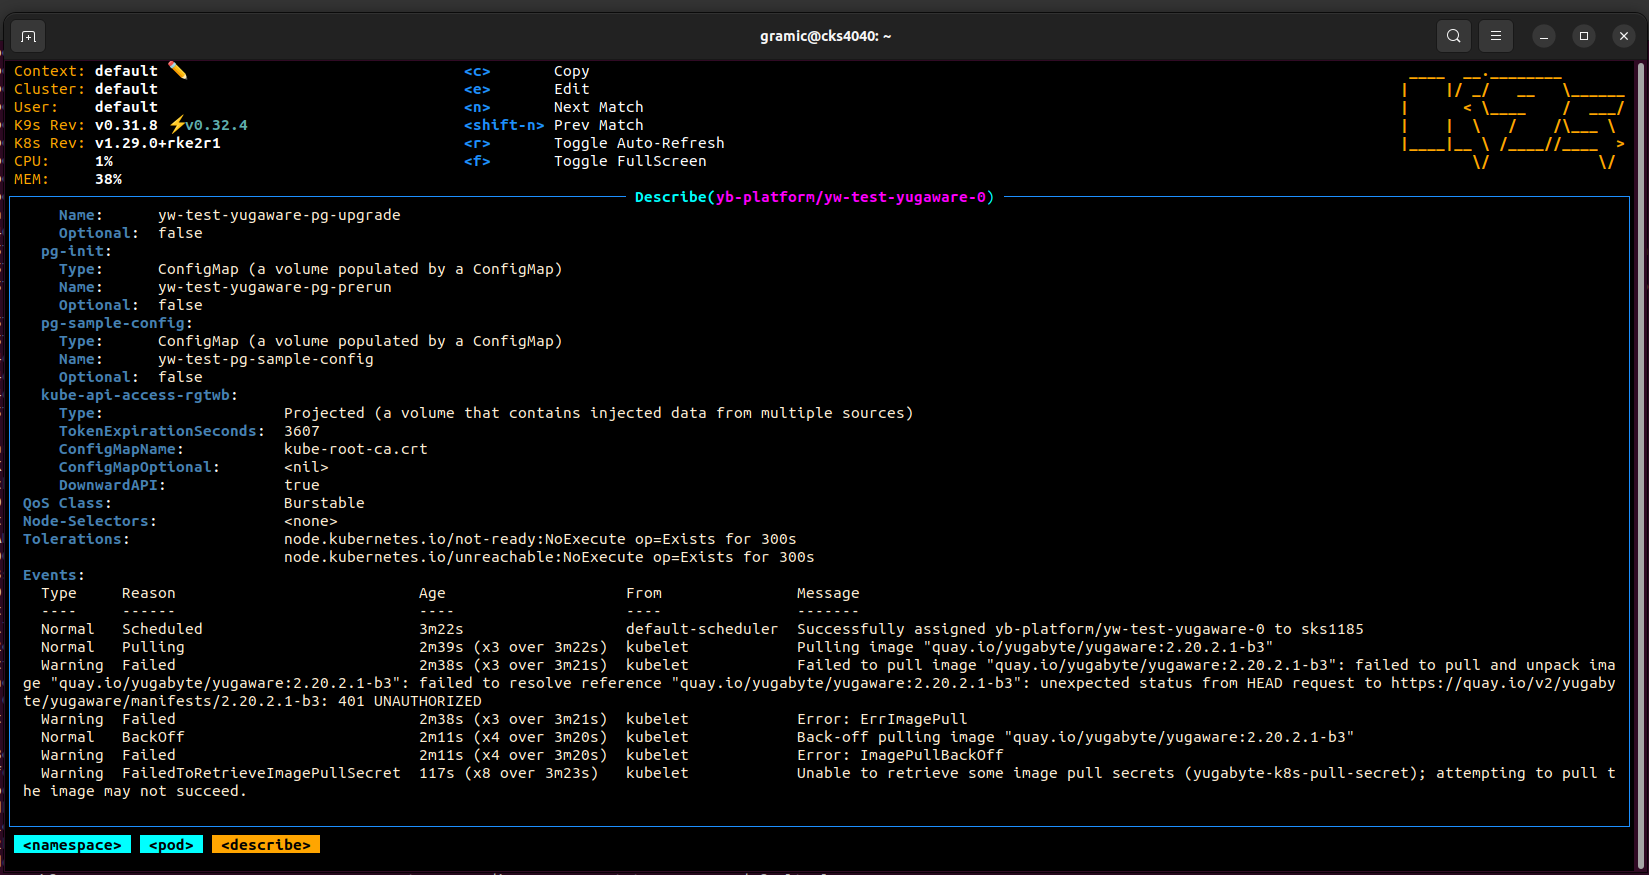
\includegraphics[width=1\linewidth]{source/implementation/evaluation/platforms/yugabytedb_pod_installation_subscription_interrup}
        \caption{yugabyteDB - Susbsription yugawre}
        \label{fig:yugabytedb_pod_installation_subscription_interrup}
    \end{figure}
\end{flushleft}
\begin{flushleft}
    Es stellte sich auch heraus, dass wenn man YugabyteDB 4 Cores pro Node zur Verfügung geben will (je zwei für den \texttt{master} und \texttt{tserver}),\\
    der Server mehr als 4 Cores haben muss.\\
    Andernfalls wird Kubernetes einen der beiden Pods nicht deployen, weil zuwenig Cores zur verfügung stehen.
\end{flushleft}
\begin{flushleft}
    Bei der konstelation \gls{rke2}, \Gls{Cilium} und \Gls{MetalLB}, muss nebst dem \texttt{IPAddressPool} auch ein \texttt{L2Advertisement} für den Pool gesetzt werden.\\
    Ansonsten kann die im YugabyteDB values.yaml gesetzte IP für den \texttt{tserver} von aussen nicht angesprochen werden:
    \lstset{style=gra_codestyle}
    \begin{lstlisting}[language=yaml, caption=metallb - Konfig YAML - Detail L2Advertisement,captionpos=b,label={lst:metallb-l2advertisement-setting},breaklines=true]
---
apiVersion: metallb.io/v1beta1
kind: L2Advertisement
metadata:
  name: l2adv
  namespace: metallb-system
spec:
  ipAddressPools:
  - distributed-sql
    \end{lstlisting}
    Dieses Problem ist schwer zu greifen und hat zwei Tage in Anspruch genommen, es zu Lösen.
    Die Vorschläge zum Lösen des Problems reichten von deakivieren von \texttt{kube-proxy} bis hin zu einer Migration zum \Gls{Cilium}-Loadb-Balancers.\\
    Mit diesem funktionierte dann nicht einmal mehr die Installation von yugabyteDB.\\
    Lösung brachte nur ein \texttt{GitHub}-Eintrag\cite{D4IZIEFN}, wo oben genannter Ansatz empfohlen wurde.
\end{flushleft}
\begin{flushleft}
    \paragraph{Konfiguration}
    Damit nicht der YugabyteDB Anywhere-Service installiert wird, muss das entsprechende Image gesetzt werden:
    \lstset{style=gra_codestyle}
    \begin{lstlisting}[language=yaml, caption=yugabyteDB - Helm Chart Manifest - Detail Image,captionpos=b,label={lst:yugabytedb-image-setting},breaklines=true]
...
Image:
  repository: "yugabytedb/yugabyte"
  tag: 2.20.2.1-b3
  pullPolicy: IfNotPresent
  pullSecretName: ""
...
    \end{lstlisting}

    Die StorageClass muss im \texttt{values.yaml} gesetzt werden, einmal für den \texttt{master} und einmal für den \texttt{tserver}
    \lstset{style=gra_codestyle}
    \begin{lstlisting}[language=yaml, caption=yugabyteDB - Helm Chart Manifest - Detail StorageClass,captionpos=b,label={lst:yugabytedb-storageclass-setting},breaklines=true]
...
storage:
  ephemeral: false  # will not allocate PVs when true
  master:
    count: 1
    size: 3Gi
    storageClass: "yb-storage"
  tserver:
    count: 1
    size: 3Gi
    storageClass: "yb-storage"
...
    \end{lstlisting}

    Dem node werden je 4 Cores zur verfügung gestellt.
    Zei für den \texttt{master} und zwei für den \texttt{tserver}.
    Beide erhalten 4GiB Memory:
    \lstset{style=gra_codestyle}
    \begin{lstlisting}[language=yaml, caption=yugabyteDB - Helm Chart Manifest - Detail Resources,captionpos=b,label={lst:yugabytedb-resources-setting},breaklines=true]
...
resource:
  master:
    requests:
      cpu: "1"
      memory: 2Gi
    limits:
      cpu: "1"
      ## Ensure the 'memory' value is strictly in 'Gi' or 'G' format. Deviating from these formats
      ## may result in setting an incorrect value for the 'memory_limit_hard_bytes' flag.
      ## Avoid using floating numbers for the numeric part of 'memory'. Doing so may lead to
      ## the 'memory_limit_hard_bytes' being set to 0, as the function expects integer values.
      memory: 2Gi
  tserver:
    requests:
      cpu: "1"
      memory: 4Gi
    limits:
      cpu: "1"
      ## Ensure the 'memory' value is strictly in 'Gi' or 'G' format. Deviating from these formats
      ## may result in setting an incorrect value for the 'memory_limit_hard_bytes' flag.
      ## Avoid using floating numbers for the numeric part of 'memory'. Doing so may lead to
      ## the 'memory_limit_hard_bytes' being set to 0, as the function expects integer values.
      memory: 4Gi
...
    \end{lstlisting}

    Die Shards, oder Tablets wie sie Yugabyte nennt, sollen auf allen drei Nodes repliziert werden:
    \lstset{style=gra_codestyle}
    \begin{lstlisting}[language=yaml, caption=yugabyteDB - Helm Chart Manifest - Detail Replika,captionpos=b,label={lst:yugabytedb-replica-setting},breaklines=true]
...
replicas:
  master: 3
  tserver: 3
  ## Used to set replication factor when isMultiAz is set to true
  totalMasters: 3
...
    \end{lstlisting}

    Wichtig ist auch, dass der \texttt{YSQL}-Dienst aktiv ist, damit PostgreSQL Abfragen abgesetzt werden können.\\
    Deshalb muss der Dienst aktiv sein und darf nicht deaktiviert werden:
    \lstset{style=gra_codestyle}
    \begin{lstlisting}[language=yaml, caption=yugabyteDB - Helm Chart Manifest - Detail Disable YSQL,captionpos=b,label={lst:yugabytedb-disableYsql-setting},breaklines=true]
...
# Disable the YSQL
disableYsql: false
...
    \end{lstlisting}

    Nun muss die Domain und die Service-Endpoints konfiguriert werden.\\
    Der Domainname bleibt vorerst \texttt{cluster.local} wie Default hinterlegt.\\
    Die Servicenamen und Ports werden nicht angetastet, wichtig ist die LoadBalancer-IP.\\
    Sie ist entsprechend der gewählten VirtualIP mit \texttt{10.0.20.106} zu setzen.

    \lstset{style=gra_codestyle}
    \begin{lstlisting}[language=yaml, caption=yugabyteDB - Helm Chart Manifest - Detail Domainname und Service-Endpoints,captionpos=b,label={lst:yugabytedb-domainname-serviceendpoints-setting},breaklines=true]
...
domainName: "cluster.local"

serviceEndpoints:
  - name: "yb-master-ui"
    type: LoadBalancer
    annotations: {}
    clusterIP: ""
    ## Sets the Service's externalTrafficPolicy
    externalTrafficPolicy: ""
    app: "yb-master"
    loadBalancerIP: ""
    ports:
      http-ui: "7000"

  - name: "yb-tserver-service"
    type: LoadBalancer
    annotations:
      metallb.universe.tf/loadBalancerIPs: 10.0.20.106
    clusterIP: ""
    ## Sets the Service's externalTrafficPolicy
    externalTrafficPolicy: ""
    app: "yb-tserver"
    loadBalancerIP: ""
    ports:
      tcp-yql-port: "9042"
      tcp-yedis-port: "6379"
      tcp-ysql-port: "5433"
...
    \end{lstlisting}
\end{flushleft}
\begin{flushleft}
    Beim Testen mit der höchsten Anzahl an Datensätzen zeigte sich, dass der \gls{local-path-provisioner} nicht sauber konfiguriert waren.\\
    Damit auf jedem Node die Persistence Volume Claims ausgeführt werden, müssen sie deklariert werden und in den StorageClass-Manifesten auch hinterlegt werden.\\
    Genauer muss in der \texttt{nodePathMap} folgende konfiguration vorgenommen werden:
\lstset{style=gra_codestyle}
\begin{lstlisting}[language=yaml, caption=local-path-provisioner nodePathMap,captionpos=b,label={lst:local-path-provisioner_nodePathMap},breaklines=true]
...
                "nodePathMap":[
                {
                        "node":"DEFAULT_PATH_FOR_NON_LISTED_NODES",
                        "paths":["<Lokaler Pfad>"]
                },
                {
                        "node":"<Nodename>",
                        "paths":["<Lokaler Pfad>"]
                },
...
\end{lstlisting}
    Hier ein Beispiel wie es mit den grossen Volumes aussieht:
\lstset{style=gra_codestyle}
\begin{lstlisting}[language=yaml, caption=local-path-provisioner nodePathMap Beispiel,captionpos=b,label={lst:local-path-provisioner_nodePathMap-exampl},breaklines=true]
...
                "nodePathMap":[
                {
                        "node":"DEFAULT_PATH_FOR_NON_LISTED_NODES",
                        "paths":["/srv/data/local-path-provisioner"]
                },
                {
                        "node":"sks1183",
                        "paths":["/srv/data/local-path-provisioner"]
                },
                {
                        "node":"sks1184",
                        "paths":["/srv/data/local-path-provisioner"]
                },
                {
                        "node":"sks1185",
                        "paths":["/srv/data/local-path-provisioner"]
                }
                ]
...
\end{lstlisting}
    Wird dies nicht gemacht, so wird auf den Default-Path geschrieben.\\
    Das ist zufällig und hat dann zur Folge, dass alle Volumes auf einem Node präsentiert werden.\\
    Was sehr schnell logischerweise dazu führt, dass zuwenig Diskspace vorhanden ist.\\
    Bei YugabyteDB kommt noch dazu, dass es zu Konflikten beim Schreiben von Blocks kommt.
\end{flushleft}
\begin{flushleft}
    Damit die Persistence Volumes sauber präsentiert werden, muss in der StorageClass die \texttt{nodeAffinity} gesetzt werden.\\
    Hier als Beispiel mit den Nodes \texttt{sks1183}, \texttt{sks1184} und \texttt{sks1185}:
\lstset{style=gra_codestyle}
\begin{lstlisting}[language=yaml, caption=yugabyteDB - StorageClass nodeAffinity,captionpos=b,label={lst:yugabytedb-storageclass_example},breaklines=true]
  nodeAffinity:
    required:
      nodeSelectorTerms:
      - matchExpressions:
        - key: kubernetes.io/hostname
          operator: In
          values:
          - sks1183
          - sks1184
          - sks1185
\end{lstlisting}
    \begin{warning}
        \textbf{hostPath}\\
        Der \texttt{hostPath} bei der StorageClass muss der gleiche sein, wie der Pfad im Node des nodePathMap von \gls{local-path-provisioner}.
        Auch sollten die Pfade auf allen Nodes gleich sein.
    \end{warning}
\end{flushleft}
\begin{flushleft}
    Die Problematik mit dem \texttt{nodePathMap} und der \texttt{nodeAffinity} auf der StorageClass hat auch rund zwei Arbeitstage in Anspruch genommen.
\end{flushleft}
    \subsubsection{Stackgres mit Citus}
\begin{flushleft} 
Stackgres ist eine PostgreSQL Implementation die dafür vorgesehenen ist, in einem Kubernetes Cluster betrieben zu werden.
\end{flushleft} 
\begin{flushleft}
An sich wäre Stackgres nur eine Implementation von Patroni in Kubernetes inkl. Load Balancer.\\
Nun kommt das Citus-Plugin ins spiel, welches aus einer jeden Monolithischen, Klassischen PostgreSQL Installation eine Distributed SQL Umgebung macht.////
Citus wiederum ist in den Microsoft Konzern eingebettet
\end{flushleft}

\begin{flushleft}
    \paragraph{Architektur}
    \begin{flushleft}
        \subparagraph{Citus Coordinator und Workers}
        \begin{figure}[H]
            \centering
            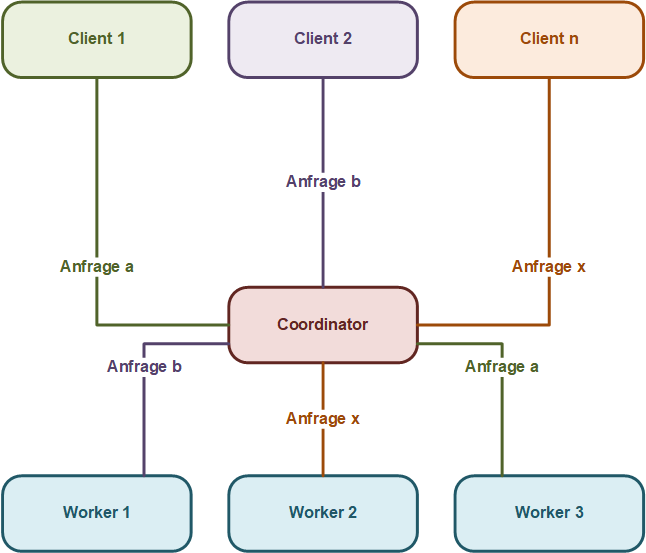
\includegraphics[width=0.75\linewidth]{source/implementation/evaluation/postgresql_ha_solutions/stackgres/citus_coordinator_worker}
            \caption{Citus - Coordinator und Workers}
            \label{fig:citus_coordinator_worker}
        \end{figure}
    \end{flushleft}
    \begin{flushleft}
        \subparagraph{Citus Sharding}
        Citus bietet zwei Sharding-Modelle an.
        \begin{flushleft}
            \textbf{Row-based sharding}
            Beim diesen sharding werden Tabellen anhand einer Distribution Column aufgeteilt. \cite{2Y5FA36C, FDUUL9IM}
        \end{flushleft}
        \begin{flushleft}
            \textbf{Schema-based sharding}
        \end{flushleft}
    \end{flushleft}
\end{flushleft}
\begin{flushleft}
    \paragraph{Maintenance}
    Bei Stackgres gab es im letzten Monat keine wirkliche Bewegung:
    \begin{figure}[H]
        \centering
        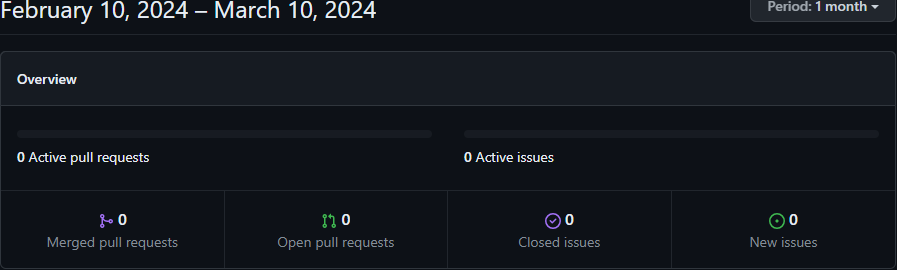
\includegraphics[width=0.75\linewidth]{source/implementation/evaluation/postgresql_ha_solutions/insights/stackgres_citus/pulse_ongres_stackgres}
        \caption{Stackgres - Pulse}
        \label{fig:pulse_ongres_stackgres}
    \end{figure}
    Anders sieht es bei Citus aus, die Firma die mittlerweile zu Microsoft gehört, schliesst Issues rasch und hat eine verhältnissmässig hohe Requstrate:
    \begin{figure}[H]
        \centering
        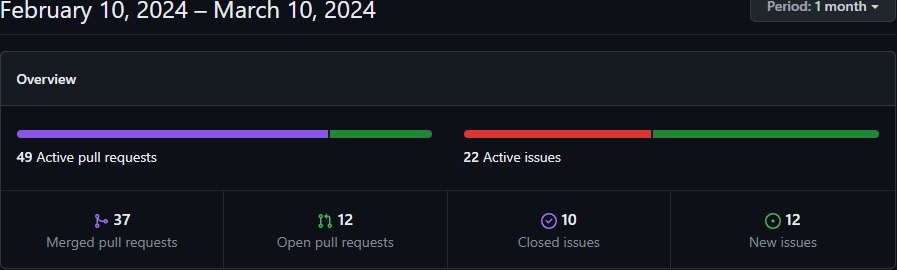
\includegraphics[width=0.75\linewidth]{source/implementation/evaluation/postgresql_ha_solutions/insights/stackgres_citus/pulse_citusdata_citus}
        \caption{Citus - Pulse}
        \label{fig:pulse_citusdata_citus}
    \end{figure}

    Bei Stackgres wird sehr viel Code hinzugefügt oder gelöscht, beim älteren Citus wurden weniger änderungen verzeichnet:
    \begin{figure}[H]
        \centering
        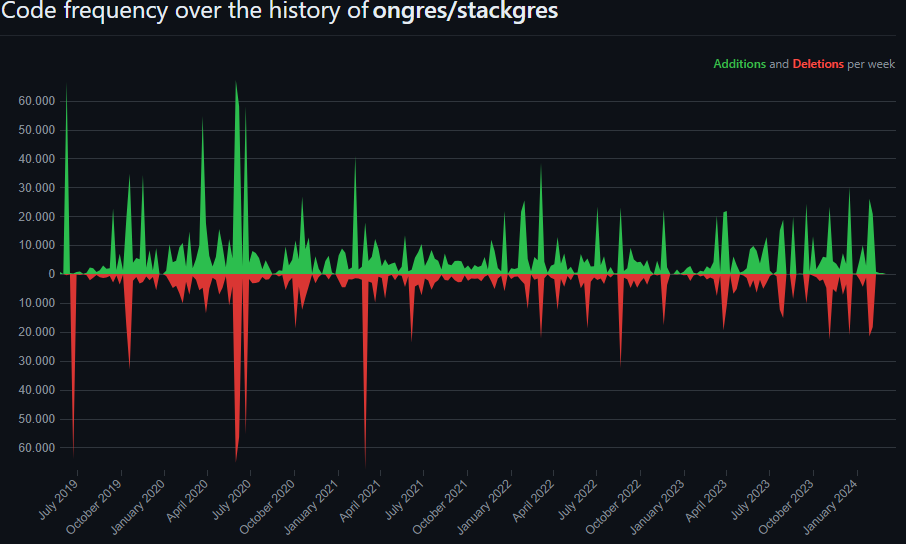
\includegraphics[width=0.75\linewidth]{source/implementation/evaluation/postgresql_ha_solutions/insights/stackgres_citus/code_frequency_ongres_stackgres}
        \caption{Stackgres - Code Frequency}
        \label{fig:code_frequency_ongres_stackgres}
    \end{figure}
    \begin{figure}[H]
        \centering
        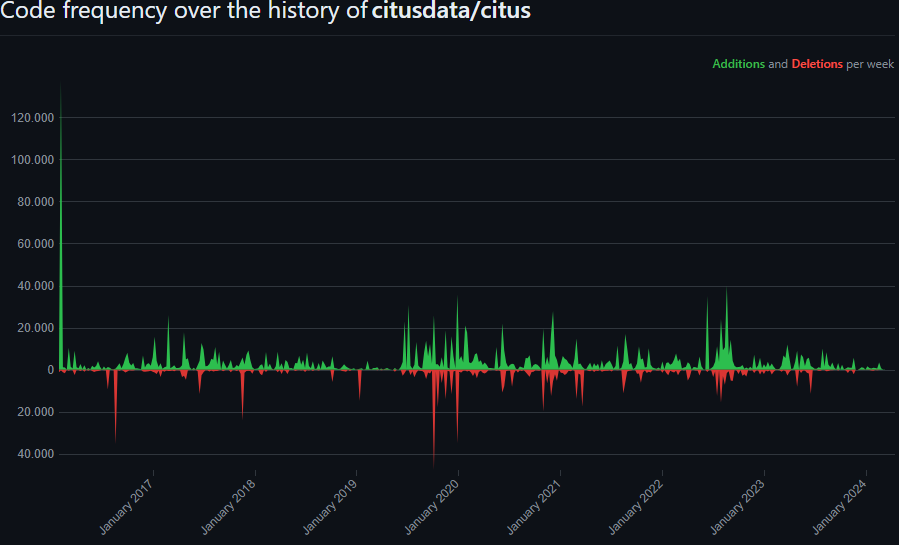
\includegraphics[width=0.75\linewidth]{source/implementation/evaluation/postgresql_ha_solutions/insights/stackgres_citus/code_frequency_citusdata_citus}
        \caption{Citus - Code Frequency}
        \label{fig:code_frequency_citusdata_citus}
    \end{figure}

    Citus legt einen hohen Stellenwert auf die Community-Standars, Stackgres selbst schneidet hier nur Mittelmässig ab:
    \begin{figure}[H]
        \centering
        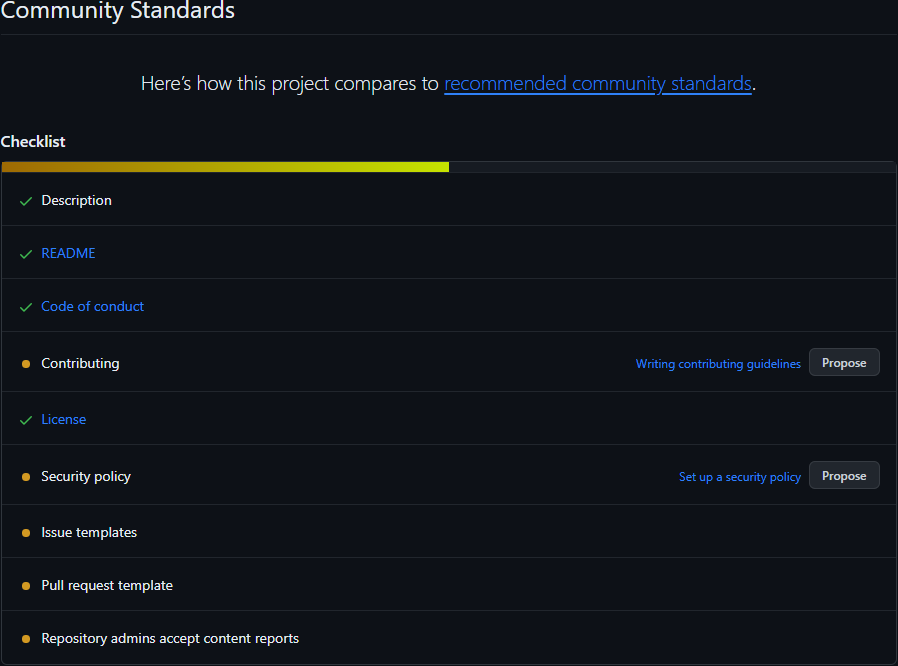
\includegraphics[width=0.75\linewidth]{source/implementation/evaluation/postgresql_ha_solutions/insights/stackgres_citus/stackgres_community_standards}
        \caption{Stackgres - Community Standards}
        \label{fig:stackgres_community_standards}
    \end{figure}
    \begin{figure}[H]
        \centering
        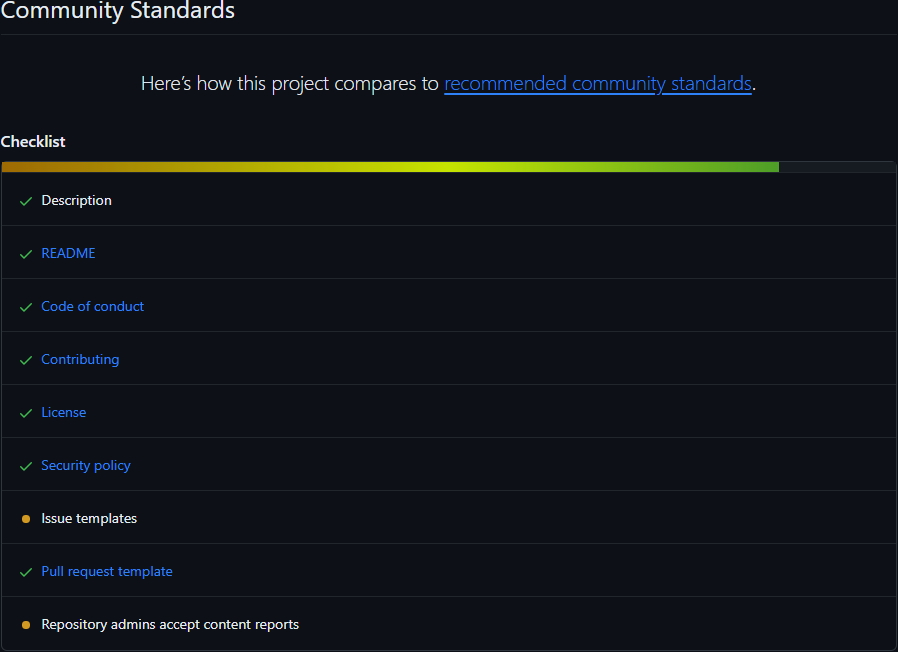
\includegraphics[width=0.75\linewidth]{source/implementation/evaluation/postgresql_ha_solutions/insights/stackgres_citus/citus_community_standards}
        \caption{Citus - Community Standards}
        \label{fig:citus_community_standards}
    \end{figure}

    Die Stackgres Constributors pflegen aktiv Additions ein, löschen Regelmässig und Commiten ebenfalls auf die main-Branch.
    Citus, dessen Repository länger Commited wird, hat weniger bewegung auf die main-Branch.
    \begin{figure}[H]
        \centering
        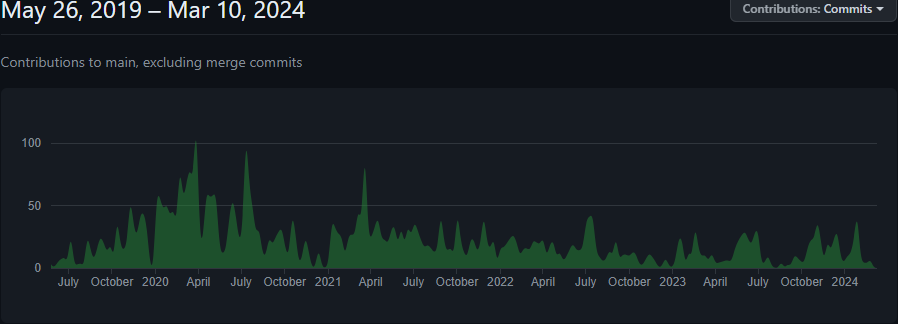
\includegraphics[width=0.75\linewidth]{source/implementation/evaluation/postgresql_ha_solutions/insights/stackgres_citus/contributors_commits_ongres_stackgres}
        \caption{Stackgres - Contributors Commits}
        \label{fig:contributors_commits_ongres_stackgres}
    \end{figure}
    \begin{figure}[H]
        \centering
        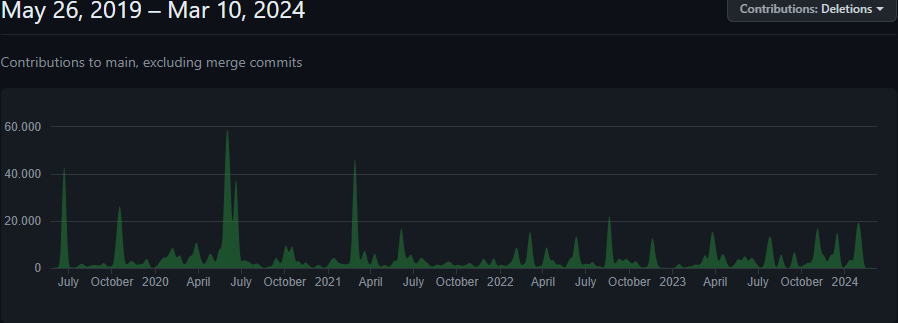
\includegraphics[width=0.75\linewidth]{source/implementation/evaluation/postgresql_ha_solutions/insights/stackgres_citus/contributors_deletations_ongres_stackgres}
        \caption{Stackgres - Contributors Deletations}
        \label{fig:contributors_deletations_ongres_stackgres}
    \end{figure}
    \begin{figure}[H]
        \centering
        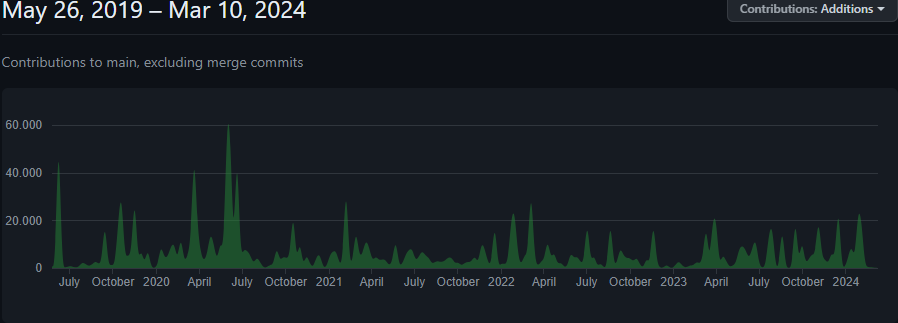
\includegraphics[width=0.75\linewidth]{source/implementation/evaluation/postgresql_ha_solutions/insights/stackgres_citus/contributors_addition_ongres_stackgres}
        \caption{Stackgres - Contributors Additions}
        \label{fig:contributors_addition_ongres_stackgres}
    \end{figure}
    \begin{figure}[H]
        \centering
        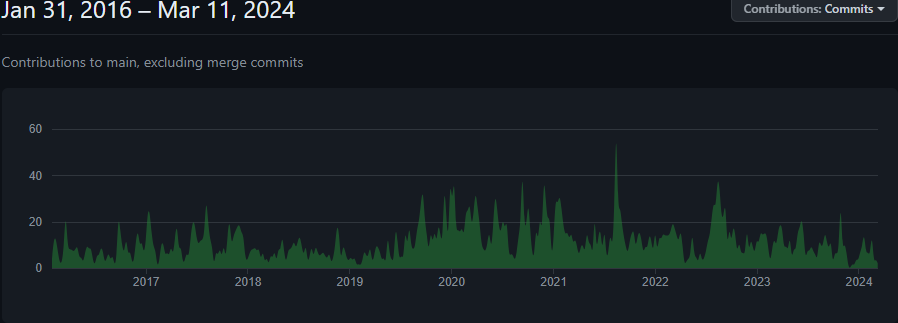
\includegraphics[width=0.75\linewidth]{source/implementation/evaluation/postgresql_ha_solutions/insights/stackgres_citus/contributors_commits_citusdata_citus}
        \caption{Citus - Contributors Commits}
        \label{fig:contributors_commits_citusdata_citus}
    \end{figure}
    \begin{figure}[H]
        \centering
        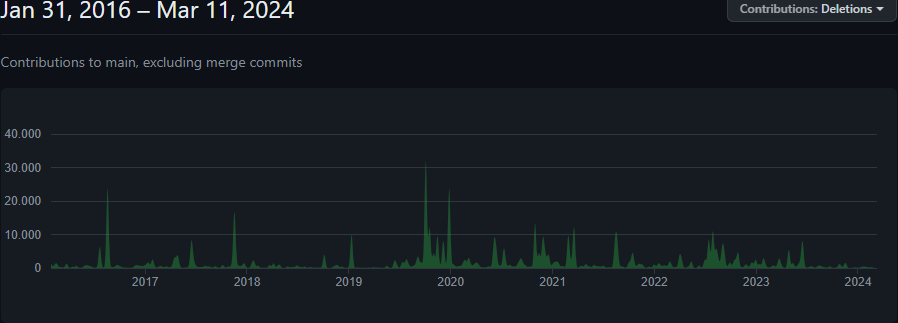
\includegraphics[width=0.75\linewidth]{source/implementation/evaluation/postgresql_ha_solutions/insights/stackgres_citus/contributors_deletations_citusdata_citus}
        \caption{Citus - Contributors Deletations}
        \label{fig:contributors_deletations_citusdata_citus}
    \end{figure}
    \begin{figure}[H]
        \centering
        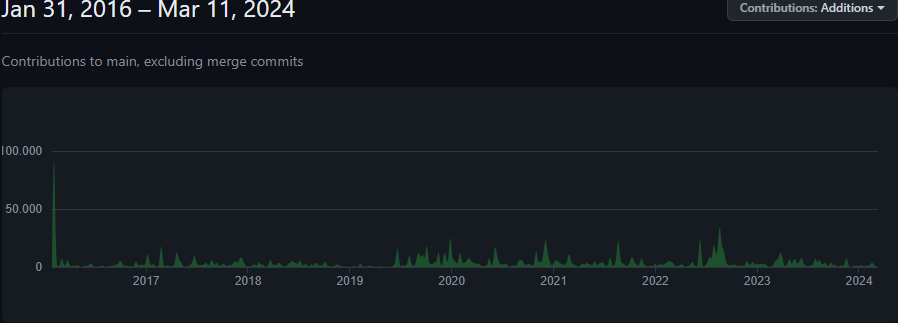
\includegraphics[width=0.75\linewidth]{source/implementation/evaluation/postgresql_ha_solutions/insights/stackgres_citus/contributors_additions_citusdata_citus}
        \caption{Citus - Contributors Additions}
        \label{fig:contributors_additions_citusdata_citus}
    \end{figure}

    Gerade Ende Januar gab es bei Stackgres eine grössere Anzahl Commits, anhand der statistik wird ersichtlich, dass i.d.R. einmal pro Monat grössere Mengen an Commits eingespielt werden.
    Bei Citus gibt es ebenfalls Regelmässig grössere Mengen an Commits, allerdings scheint bei citusdata mehr mit kürzeren Sprints gearbeitet zu werden als bei ongres denn die Commits sind Regelmässiger:
    \begin{figure}[H]
        \centering
        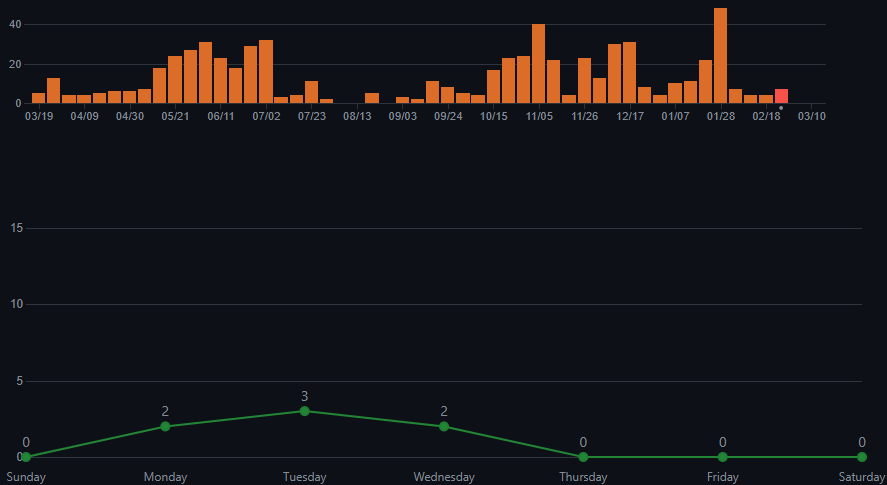
\includegraphics[width=0.75\linewidth]{source/implementation/evaluation/postgresql_ha_solutions/insights/stackgres_citus/commit_activity_ongres_stackgres}
        \caption{Stackgres - Commit Activity}
        \label{fig:commit_activity_ongres_stackgres}
    \end{figure}
    \begin{figure}[H]
        \centering
        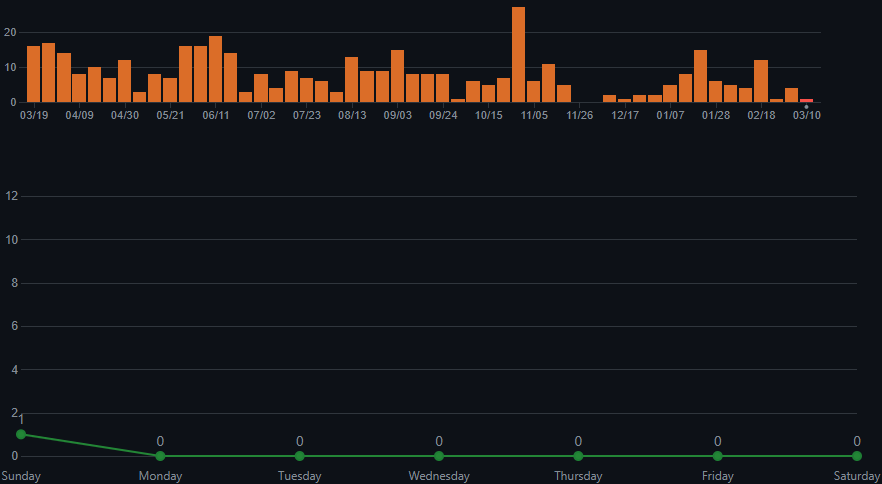
\includegraphics[width=0.75\linewidth]{source/implementation/evaluation/postgresql_ha_solutions/insights/stackgres_citus/commit_activity_citusdata_citus}
        \caption{Citus - Commit Activity}
        \label{fig:commit_activity_citusdata_citus}
    \end{figure}

    In letzter Zeit haben nur ongres, der Entwickler von Stackgres, als auch citusdata, grössere Commits auf das Repository gefahren.
    Andere grössere Entwickler wie EnterpriseDB sind abwesend.
    \begin{figure}[H]
        \centering
        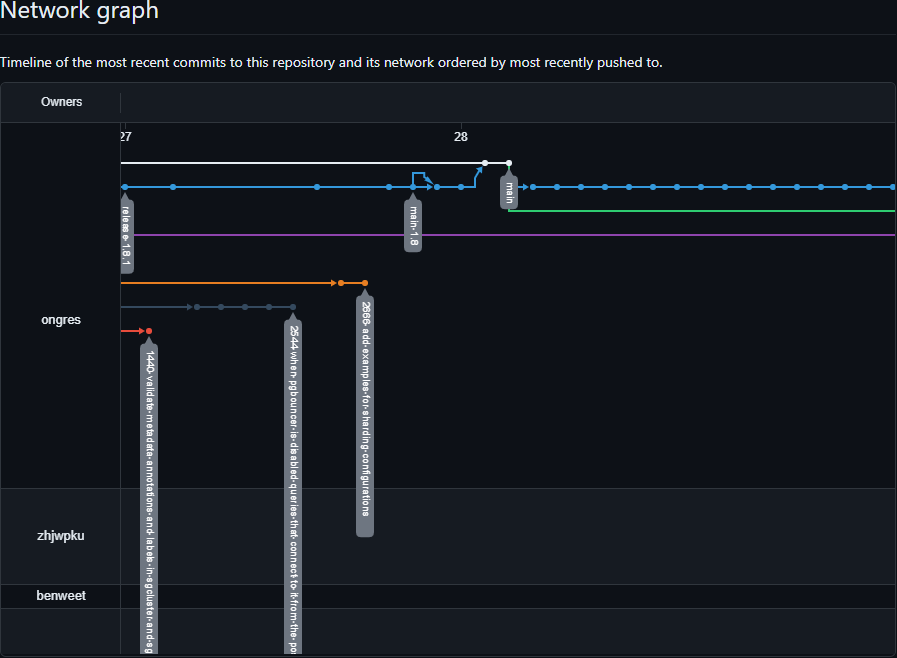
\includegraphics[width=0.75\linewidth]{source/implementation/evaluation/postgresql_ha_solutions/insights/stackgres_citus/network_graph_ongres_stackgres}
        \caption{Stackgres - Network Graph}
        \label{fig:network_graph_ongres_stackgres}
    \end{figure}
    \begin{figure}[H]
        \centering
        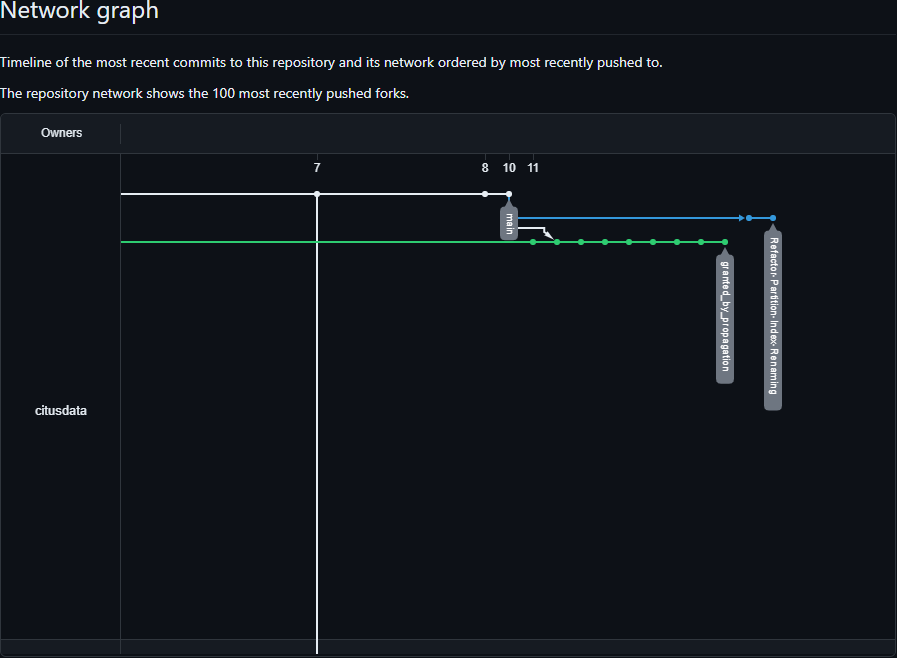
\includegraphics[width=0.75\linewidth]{source/implementation/evaluation/postgresql_ha_solutions/insights/stackgres_citus/network_graph_citusdata_citus}
        \caption{Citus - Network Graph}
        \label{fig:network_graph_citusdata_citus}
    \end{figure}

\end{flushleft}

    %! Author = itgramic
%! Date = 05.01.24

% Preamble
\newpage
\section{Disposition}
\label{chap:disposition}
%\begin{flushleft}
%    \begin{figure}[H]
%        \centering
%%        
\includegraphics[width=1\linewidth]{source/appendix/Michael_Graber_Disposition_Diplomarbeit_2023_2024}
%        
\includepdf[pages={1-},scale=0.75]{source/appendix/Michael_Graber_Disposition_Diplomarbeit_2023_2024}
%        \caption{Disposition}
%        \label{fig:disposition}
%    \end{figure}

\includepdf[pages={1-},scale=0.75]{source/appendix/Michael_Graber_Disposition_Diplomarbeit_2023_2024}
%\caption{Disposition}
%\label{fig:disposition}
\captionof{figure}{Disposition}
%\end{flushleft}

\end{appendix}

